\section{Prototipação de Baixa Fidelidade}\label{apdx:lofi}

\subsection{Cenário Textual}

Ao não se sentir bem, um usuário busca na internet por um sistema de diagnóstico online.
Esse usuário sabe que simplesmente buscar por sintomas de maneira isolada não leva a dados concretos.

Nesse contexto, este usuário encontra o sistema HealthWeb, onde, após concordar com os termos de uso, preenche alguns dados simples, como sexo, idade e peso, então segue para um questionário com perguntas do tipo sim e não a respeito de sintomas que tem ou teve desde que começou a se sentir mal.

Em seguida, uma lista de possíveis diagnósticos baseados nos sintomas, ordenados por probabilidade, começando pelo mais provável. Cada item da lista pode ser selecionado, apresentando uma pequena página com informações a respeito dessa doença, com a possibilidade de acessar a página completa a respeito desta doença.

\subsection{Proposta de logomarca}

A logomarca proposta, apresentada na figura \ref{fig:logomarca}, consiste no título ``HealthWeb'' tipografado em fonte ``Cinzel Decorative''.

\begin{figure}[hbtp]
	\centering
	
\includegraphics[width=\textwidth]{figure/logo.png}
	\caption{Logomarca proposta.}
	\label{fig:logomarca}
\end{figure}

\subsection{Tarefas realizadas pelos sistema}

Este sistema realiza a seguinte lista de tarefas:
\begin{itemize}
	\item Transitar entre páginas de informações sobre o sistema;
	\item Listar e detalhar doenças cadastradas no banco de dados;
	\item Coletar informações do usuário que serão utilizadas para o diagnóstico;
	\item Listar possíveis doenças, apresentando parâmetro estatístico, correlacionando os sintomas denotados com o banco de dados sobre doenças;
\end{itemize}

\subsection{Storyboard}

O desenvolvimento front-end seguiu uma marcha dando prioridade à versão \textit{mobile}, e a partir desta foi desenvolvida a versão \textit{desktop}.

\subsubsection{Versão mobile}

A interface inicial, figura \ref{fig:mobile:home}, consiste em um botão central para prossegui para a próxima página, e uma faixa superior contendo um botão na lateral esquerda, para acesso ao menu, a logomarca ao centro e um botão em formato de lâmpada na lateral direita, para possível ativação de modo escuro na interface geral.

\begin{figure}[htbp]
	\centering
	\hspace{0.24\linewidth}
	\hfill
	\begin{subfigure}{0.24\linewidth}
		\centering
		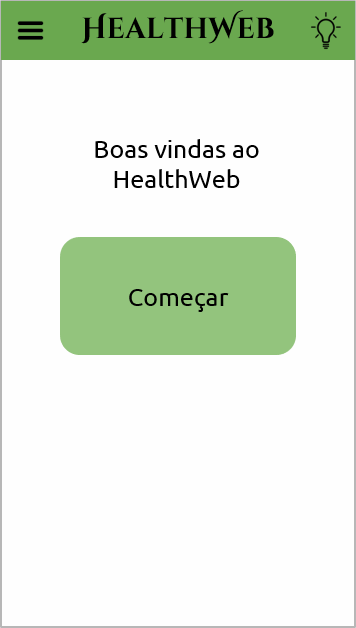
\includegraphics[width=\linewidth]{figure/prototype/mobile/home.png}
		\caption{Tela de início.}
		\label{fig:mobile:home}
	\end{subfigure}
	\hfill
	\begin{subfigure}{0.24\linewidth}
		\centering
		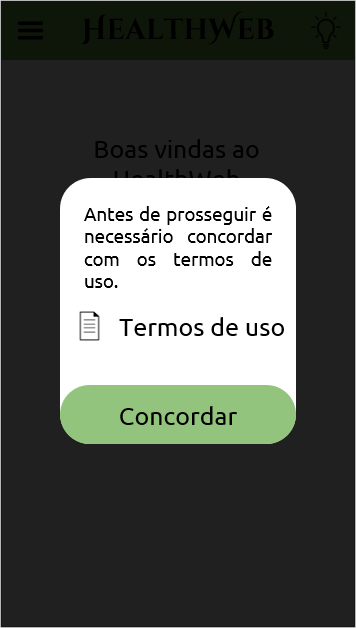
\includegraphics[width=\linewidth]{figure/prototype/mobile/agreeing.png}
		\caption{Concordar com termos.}
		\label{fig:mobile:agreeing}
	\end{subfigure}
	\hfill
	\hspace{0.24\linewidth}
	\label{fig:mobile:home_agreeing}
	\caption{Interface Inicial.}
\end{figure}

Pressionando o botão central da página inicial, surge uma janela central, figura \ref{fig:mobile:agreeing}, contendo o texto ``Antes de prosseguir é necessário concordar com os temos de uso.'', logo abaixo um link de acesso para os termos de uso. Ao final da janela um botão para concordar com os termos e prosseguir.

Acessando o menu lateral através do botão, a interface apresentada na figura \ref{fig:mobile:drawer} será vista, uma barra lateral, contendo uma lista de opções que levam às suas respectivas páginas: ``Início'', ``Doenças'', ``Termos de uso'' e ``Sobre''. Na base da barra é apresentada a versão do sistema.

A página ``Sobre'', figura \ref{fig:mobile:about}, apresenta informações sobre o sistema e a equipe de desenvolvimento.

A página ``Termo de uso'', figura \ref{fig:mobile:terms}, apresenta informações a respeito de privacidade de dados do usuário, entre outras informações cabíveis.

A página ``Doenças'', figura \ref{fig:mobile:list_disease}, apresenta a listagem de doenças cadastradas no sistema, cada item da lista é um botão que leva à página associada à doença.

\begin{figure}[htbp]
	\centering
	\begin{subfigure}{0.24\linewidth}
		\centering
		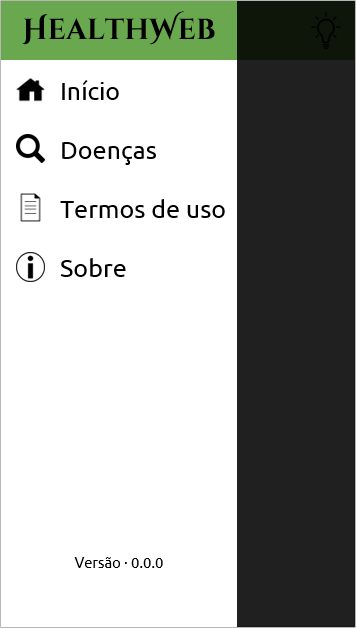
\includegraphics[width=\linewidth]{figure/prototype/mobile/drawer.png}
		\caption{Menu lateral.}
		\label{fig:mobile:drawer}
	\end{subfigure}
	\hfill
	\begin{subfigure}{0.24\linewidth}
		\centering
		
\includegraphics[width=\linewidth]{figure/prototype/mobile/about.png}
		\caption{Tela sobre.}
		\label{fig:mobile:about}
	\end{subfigure}
	\hfill
	\begin{subfigure}{0.24\linewidth}
		\centering
		
\includegraphics[width=\linewidth]{figure/prototype/mobile/terms.png}
		\caption{Tela de termos de uso.}
		\label{fig:mobile:terms}
	\end{subfigure}
	\hfill
	\begin{subfigure}{0.24\linewidth}
		\centering
		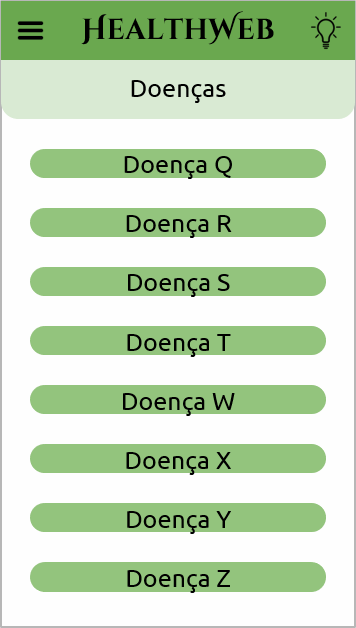
\includegraphics[width=\linewidth]{figure/prototype/mobile/list_disease.png}
		\caption{Lista de doenças.}
		\label{fig:mobile:list_disease}
	\end{subfigure}
	\caption{Menu e páginas de documentação.}
	\label{fig:mobile:drawer_about_terms_list_disease}
\end{figure}

Acessando a interface de questionário, a primeira página exibida solicita a informação a respeito de sexo biológico, \ref{fig:mobile:bio_sex}, com uma nota de rodapé a respeito da razão pela qual esta informação é relevante para o sistema.
Nesta página, apresentam-se quatro botões, ``Masculino'' e ``Feminino'', na altura central da interface e distribuídos em lados opostos da tela.
Logo abaixo, os botões ``Voltar'' e ``Continuar'', sendo o segundo desativado até que o usuário selecione uma opção de resposta para o sistema.
No espaço restante é apresentado uma barra visual de progresso, contendo também seu valor em porcentagem. Esta barra, e os botões ``Voltar'' e ``Continuar'' estão presentes em todas as telas durante o questionário.

Seguindo a rotina de respostas, a próxima tela solicita a idade do usuário, figura \ref{fig:mobile:age}, apresentando uma caixa de texto centralizada na interface.

A tela seguinte solicita a altura do usuário, figura \ref{fig:mobile:height}, a interface é equivalente à da tela anterior.

A terceira questão ao usuário é sobre seu peso, figure \ref{fig:mobile:weight}, também com interface equivalente à anterior.

\begin{figure}[htbp]
	\centering
	\begin{subfigure}{0.24\linewidth}
		\centering
		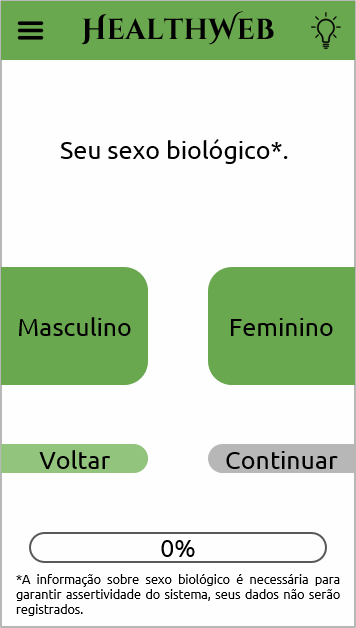
\includegraphics[width=\linewidth]{figure/prototype/mobile/bio_sex.png}
		\caption{Sexo biológico.}
		\label{fig:mobile:bio_sex}
	\end{subfigure}
	\hfill
	\begin{subfigure}{0.24\linewidth}
		\centering
		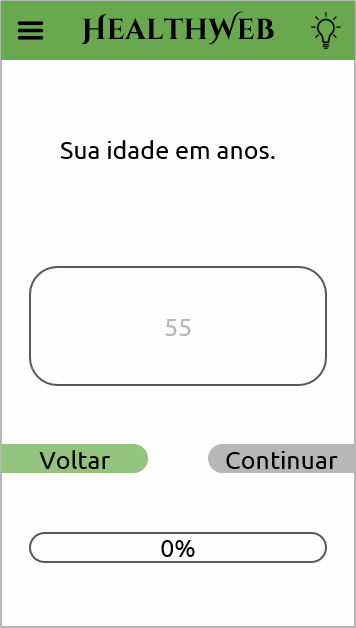
\includegraphics[width=\linewidth]{figure/prototype/mobile/age.png}
		\caption{Idade.}
		\label{fig:mobile:age}
	\end{subfigure}
	\hfill
	\begin{subfigure}{0.24\linewidth}
		\centering
		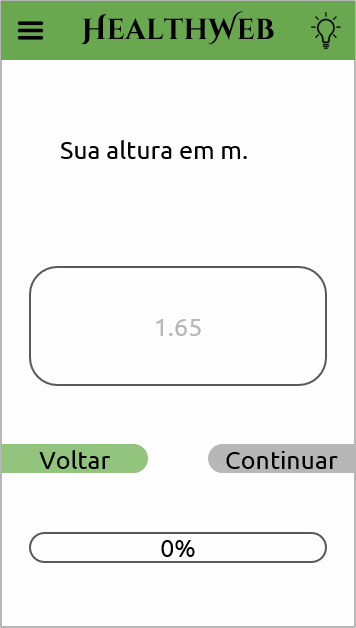
\includegraphics[width=\linewidth]{figure/prototype/mobile/height.png}
		\caption{Altura.}
		\label{fig:mobile:height}
	\end{subfigure}
	\hfill
	\begin{subfigure}{0.24\linewidth}
		\centering
		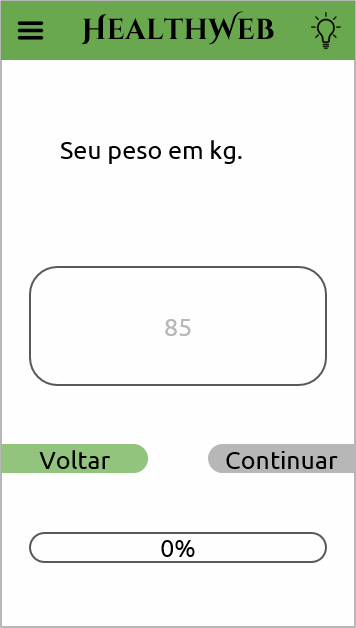
\includegraphics[width=\linewidth]{figure/prototype/mobile/weight.png}
		\caption{Peso.}
		\label{fig:mobile:weight}
	\end{subfigure}
	\caption{Perguntas sobre informações básicas do usuário.}
	\label{fig:mobile:bio_sex_age_height_weight}
\end{figure}

Chegando à interface mais presente no sistema, a tela de questionário de sintomas, figura \ref{fig:mobile:symptom}, o usuário responderá sim ou não para cada um dos sintomas apresentados. A disposição dos itens na tela é equivalente à tela de informação a respeito de sexo biológico, diferindo do conteúdo dos botões, ``Sim'' e ``Não'', e suas cores.
Quando uma opção selecionado, o botão da outra opção tem sua coloração alterada para o cinza, indicando a seleção feita, ambos aos casos são apresentados nas figuras \ref{fig:mobile:symptom_no} e \ref{fig:mobile:symptom_yes}. Após selecionada uma opção, o botão de continuar é ativado.

\begin{figure}[htbp]
	\centering
	\hspace{0.11\linewidth}
	\hfill
	\begin{subfigure}{0.24\linewidth}
		\centering
		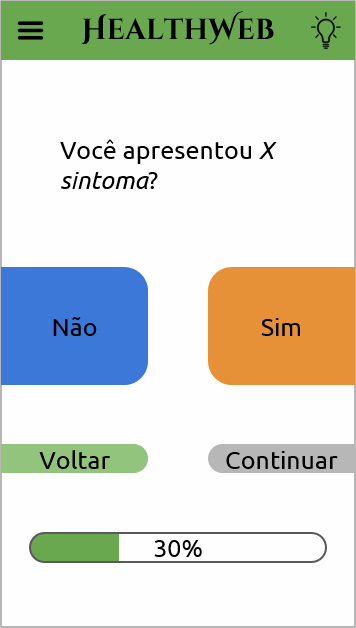
\includegraphics[width=\linewidth]{figure/prototype/mobile/symptom.png}
		\caption{Antes da resposta.}
		\label{fig:mobile:symptom}
	\end{subfigure}
	\hfill
	\begin{subfigure}{0.24\linewidth}
		\centering
		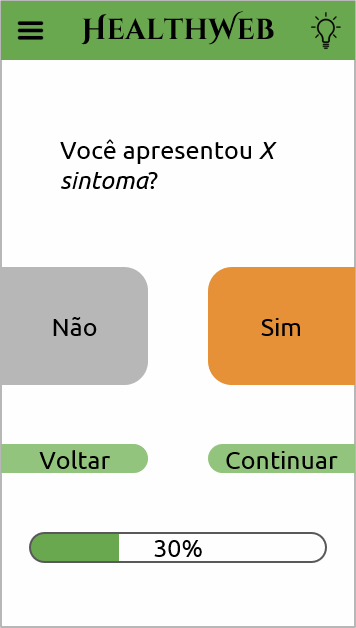
\includegraphics[width=\linewidth]{figure/prototype/mobile/symptom_yes.png}
		\caption{Resposta positiva.}
		\label{fig:mobile:symptom_yes}
	\end{subfigure}
	\hfill
	\begin{subfigure}{0.24\linewidth}
		\centering
		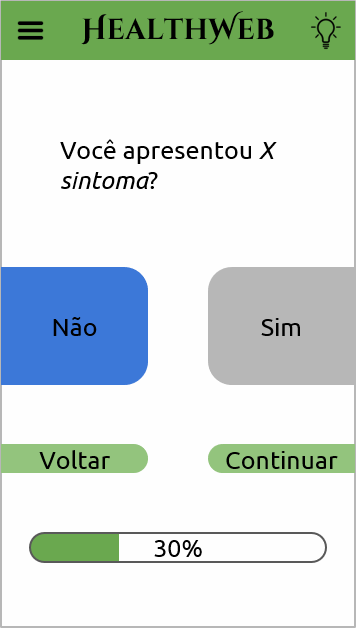
\includegraphics[width=\linewidth]{figure/prototype/mobile/symptom_no.png}
		\caption{Resposta negativa.}
		\label{fig:mobile:symptom_no}
	\end{subfigure}
	\hspace{0.11\linewidth}
	\hfill
	\caption{Interface durante questionário de sintomas.}
	\label{fig:mobile:symptom_yes_no}
\end{figure}

Depois de responder todas as perguntas a respeito de sintomas, o usuário é levado à tela de resultados, figura \ref{fig:mobile:results}, onde é apresentada uma lista das doenças mais prováveis com sua probabilidade em porcentagem, segundo as respostas. Após a lista, há um botão ``Mostrar mais'' para exibir mais resultados na lista. Logo em seguida, um botão ``O que estes resultados significam'', que leva à uma página, figure \ref{fig:mobile:meaning}, explicando o significado dos valores de porcentagem e a relevância de procurar um profissional para um diagnóstico mais preciso.

Na lista de doenças, é possível selecionar uma doença e abrir uma pequena janela com um resumo de informações a respeito, figura \ref{fig:mobile:this_disease}, à base da janela é possível acessar a página completa da doença, \ref{fig:mobile:disease_page}.

\begin{figure}[htbp]
	\centering
	\begin{subfigure}{0.24\linewidth}
		\centering
		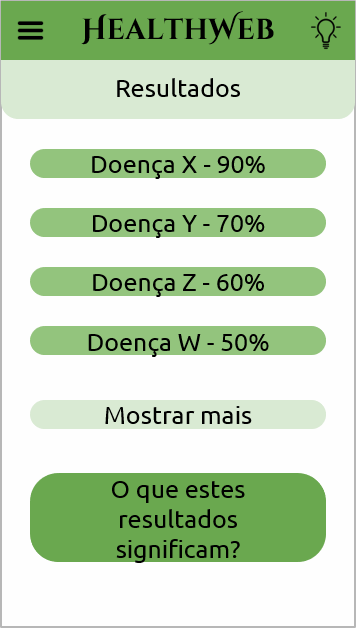
\includegraphics[width=\linewidth]{figure/prototype/mobile/results.png}
		\caption{Resultados.}
		\label{fig:mobile:results}
	\end{subfigure}
	\hfill
	\begin{subfigure}{0.24\linewidth}
		\centering
		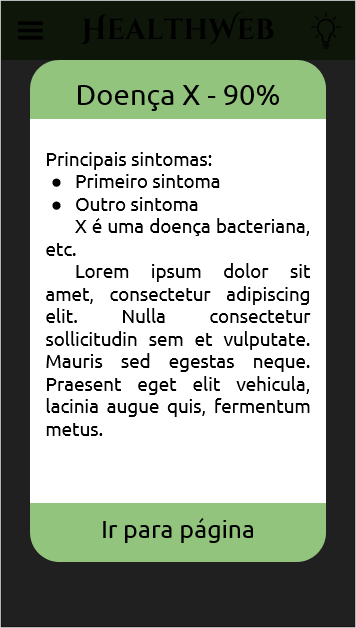
\includegraphics[width=\linewidth]{figure/prototype/mobile/this_disease.png}
		\caption{Resumo sobre doença.}
		\label{fig:mobile:this_disease}
	\end{subfigure}
	\hfill
	\begin{subfigure}{0.24\linewidth}
		\centering
		
\includegraphics[width=\linewidth]{figure/prototype/mobile/disease_page.png}
		\caption{Página sobre doença.}
		\label{fig:mobile:disease_page}
	\end{subfigure}
	\hfill
	\begin{subfigure}{0.24\linewidth}
		\centering
		
\includegraphics[width=\linewidth]{figure/prototype/mobile/meaning.png}
		\caption{Explicação.}
		\label{fig:mobile:meaning}
	\end{subfigure}
	\caption{Interface de detalhamento e resultados.}
	\label{fig:mobile:results_this_disease_disease_page_meaning}
\end{figure}

A figura \ref{fig:mobile:story} apresenta o diagrama de um \textit{storyboard} para a versão \textit{mobile} do sistema.

\begin{figure}[htbp]
	\centering
	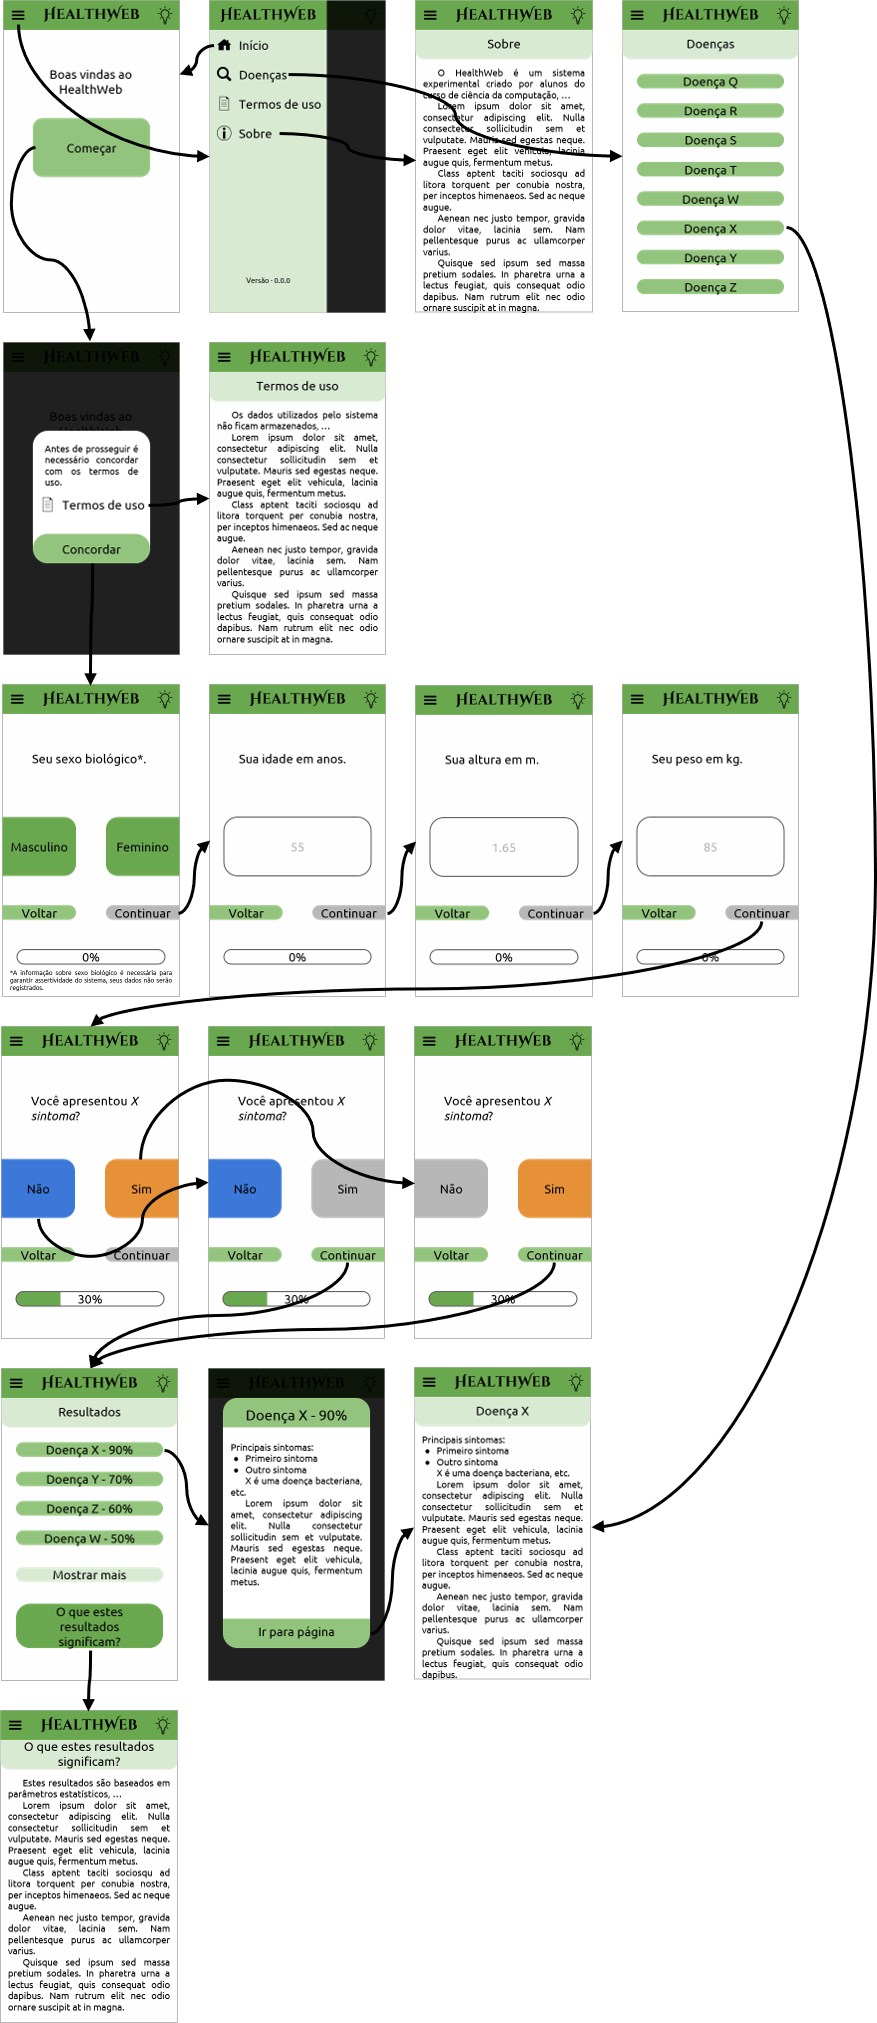
\includegraphics[width=\linewidth]{figure/prototype/mobile/storyboard.png}
	\caption{Storyboard para versão mobile.}
	\label{fig:mobile:story}
\end{figure}

\subsubsection{Versão desktop}

Todas as telas da versão \textit{mobile} estão presentes na versão \textit{desktop} com pequenas adaptações de interface.

O menu lateral, normalmente oculto na versão \textit{mobile} está normalmente presente na versão \textit{desktop}, e pode ser ocultado pelo botão de menu lateral. A figura \ref{fig:desktop:home} apresenta a interface padrão com a barra lateral, enquanto a figure \ref{fig:desktop:drawer} apresenta a interface com o menu lateral oculto.

O diagrama de \textit{storyboard} equivalente à versão \textit{desktop} está presente na figura \ref{fig:desktop:story}.

\begin{figure}[htbp]
	\centering
	\begin{subfigure}{0.49\linewidth}
		\centering
		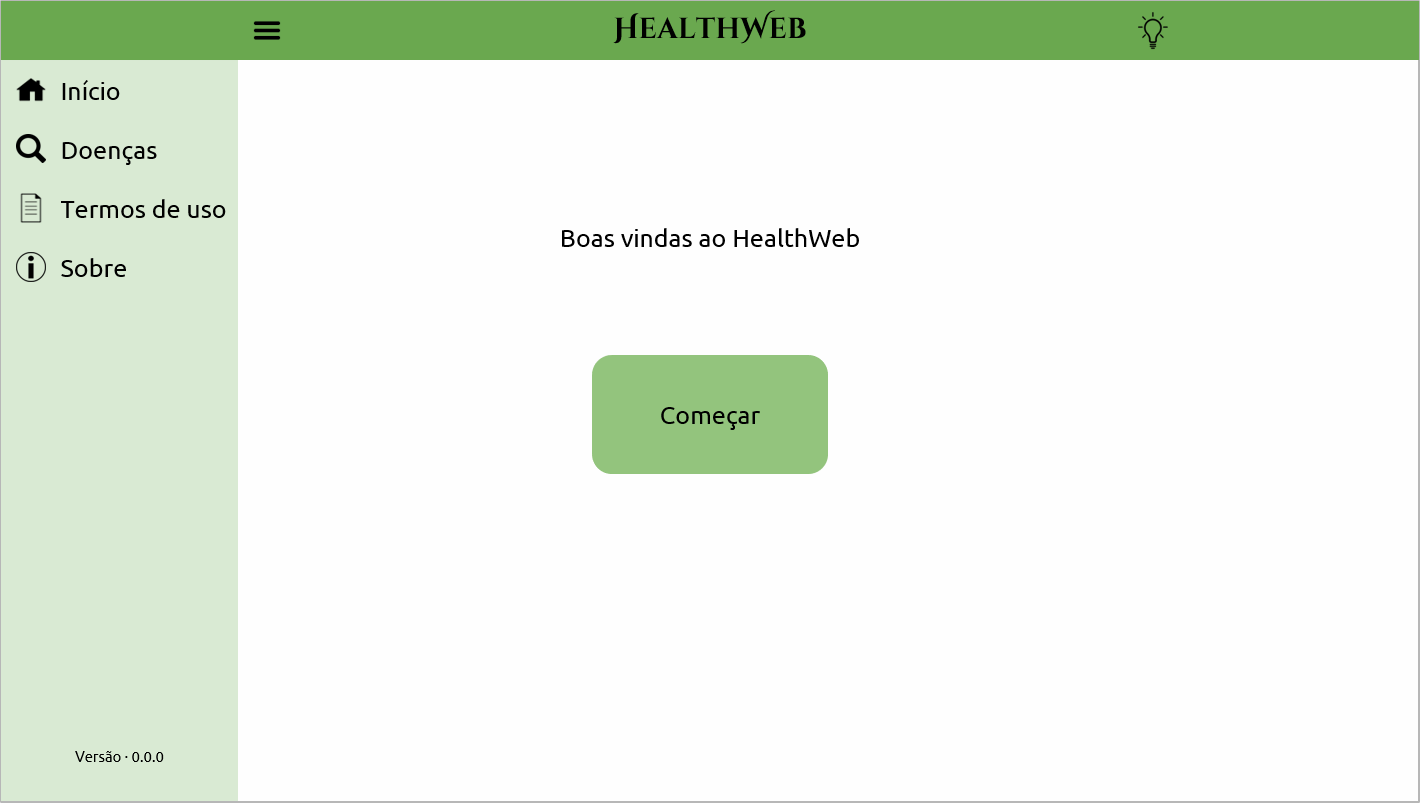
\includegraphics[width=\linewidth]{figure/prototype/desktop/home.png}
		\caption{Tela de início.}
		\label{fig:desktop:home}
	\end{subfigure}
	\hfill
	\begin{subfigure}{0.49\linewidth}
		\centering
		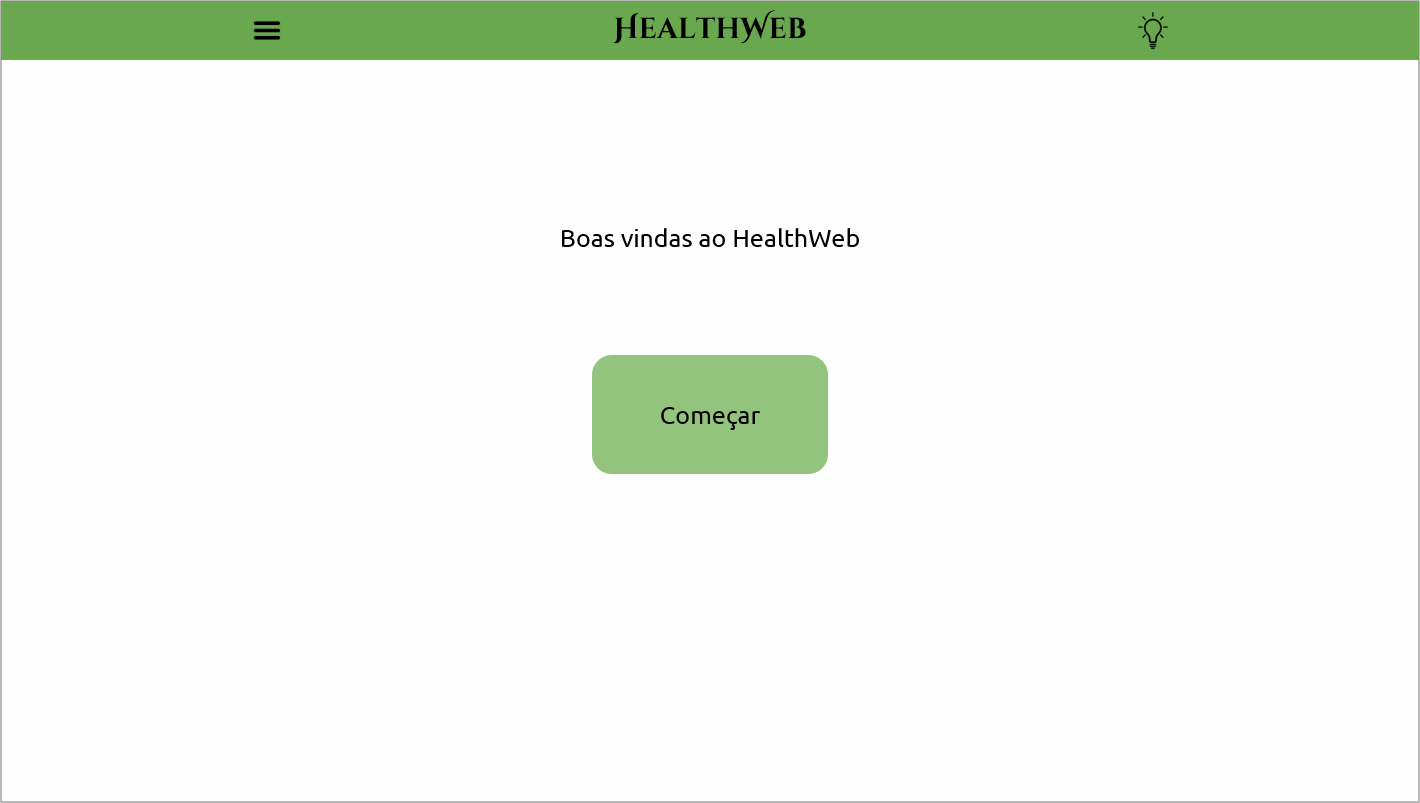
\includegraphics[width=\linewidth]{figure/prototype/desktop/drawer.png}
		\caption{Menu lateral recolhido na tela de início.}
		\label{fig:desktop:drawer}
	\end{subfigure}
	\caption{Tela de início e detalhe do menu lateral.}
	\label{fig:desktop:home_agreeing}
\end{figure}

\begin{figure}[htbp]
	\centering
	\begin{subfigure}{0.49\linewidth}
		\centering
		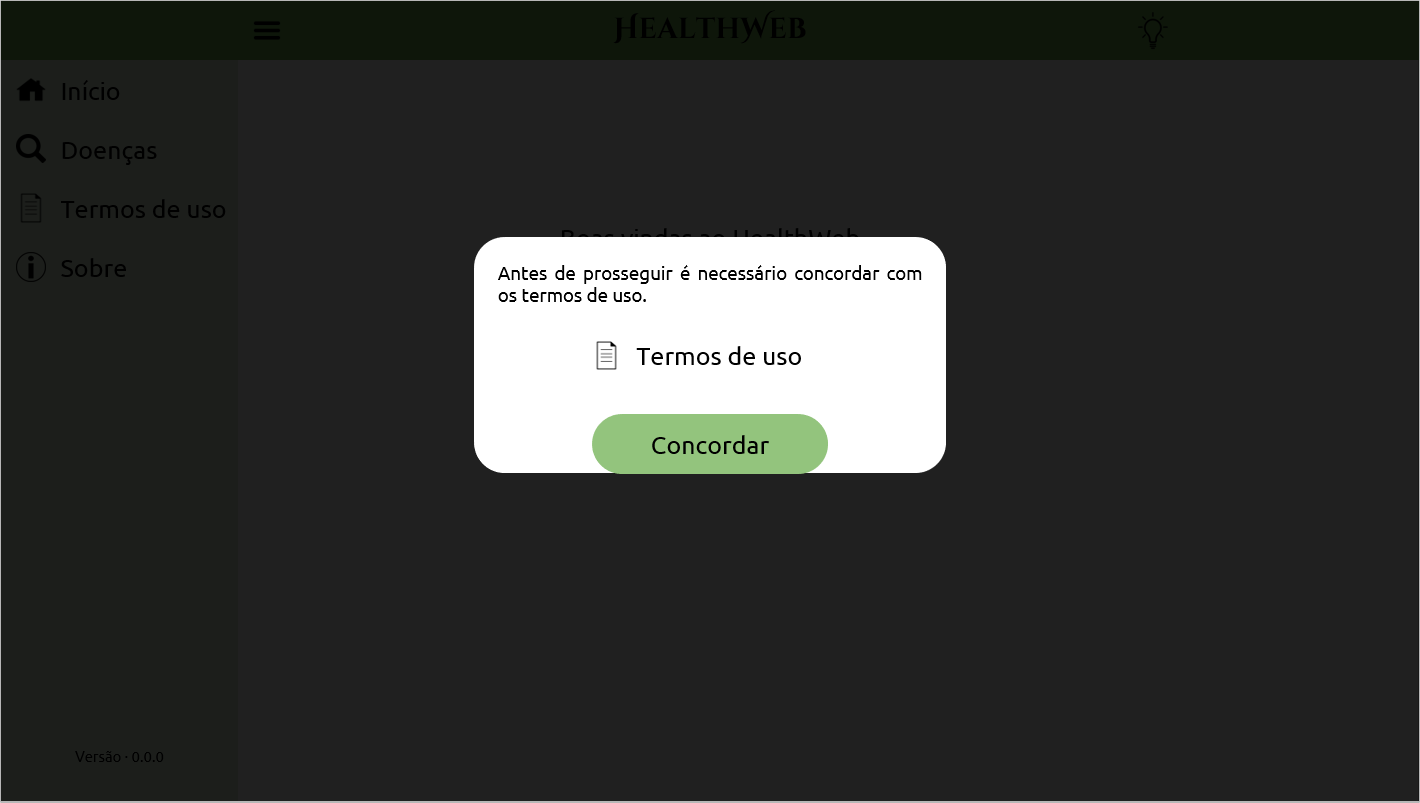
\includegraphics[width=\linewidth]{figure/prototype/desktop/agreeing.png}
		\caption{Concordar com termos.}
		\label{fig:desktop:agreeing}
	\end{subfigure}
	\hfill
	\begin{subfigure}{0.49\linewidth}
		\centering
		
\includegraphics[width=\linewidth]{figure/prototype/desktop/about.png}
		\caption{Tela sobre.}
		\label{fig:desktop:about}
	\end{subfigure}
	\hfill
	\begin{subfigure}{0.49\linewidth}
		\centering
		
\includegraphics[width=\linewidth]{figure/prototype/desktop/terms.png}
		\caption{Tela de termos de uso.}
		\label{fig:desktop:terms}
	\end{subfigure}
	\hfill
	\begin{subfigure}{0.49\linewidth}
		\centering
		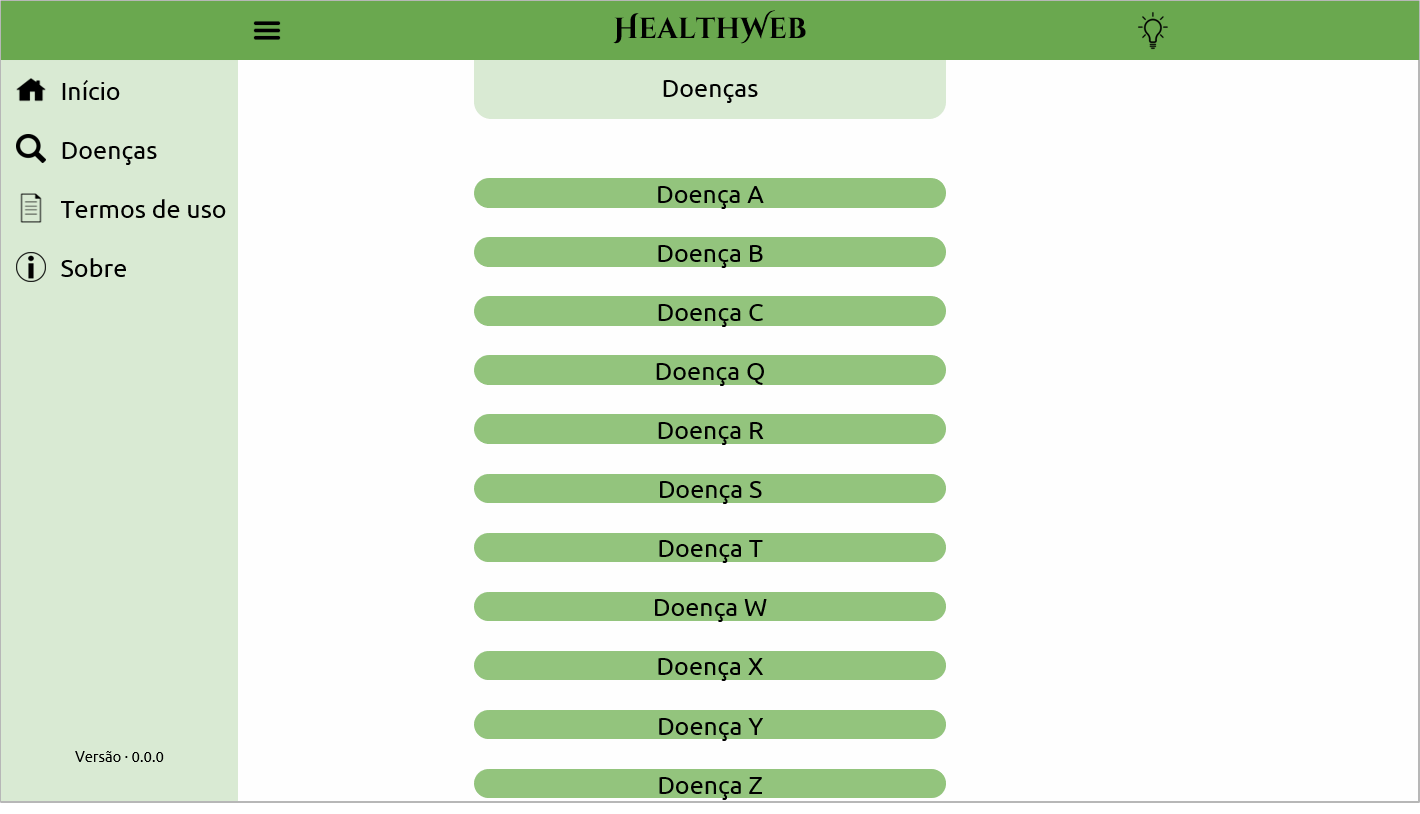
\includegraphics[width=\linewidth]{figure/prototype/desktop/list_disease.png}
		\caption{Lista de doenças.}
		\label{fig:desktop:list_disease}
	\end{subfigure}
	\caption{Páginas de documentação.}
	\label{fig:desktop:drawer_about_terms_list_disease}
\end{figure}

\begin{figure}[htbp]
	\centering
	\begin{subfigure}{0.49\linewidth}
		\centering
		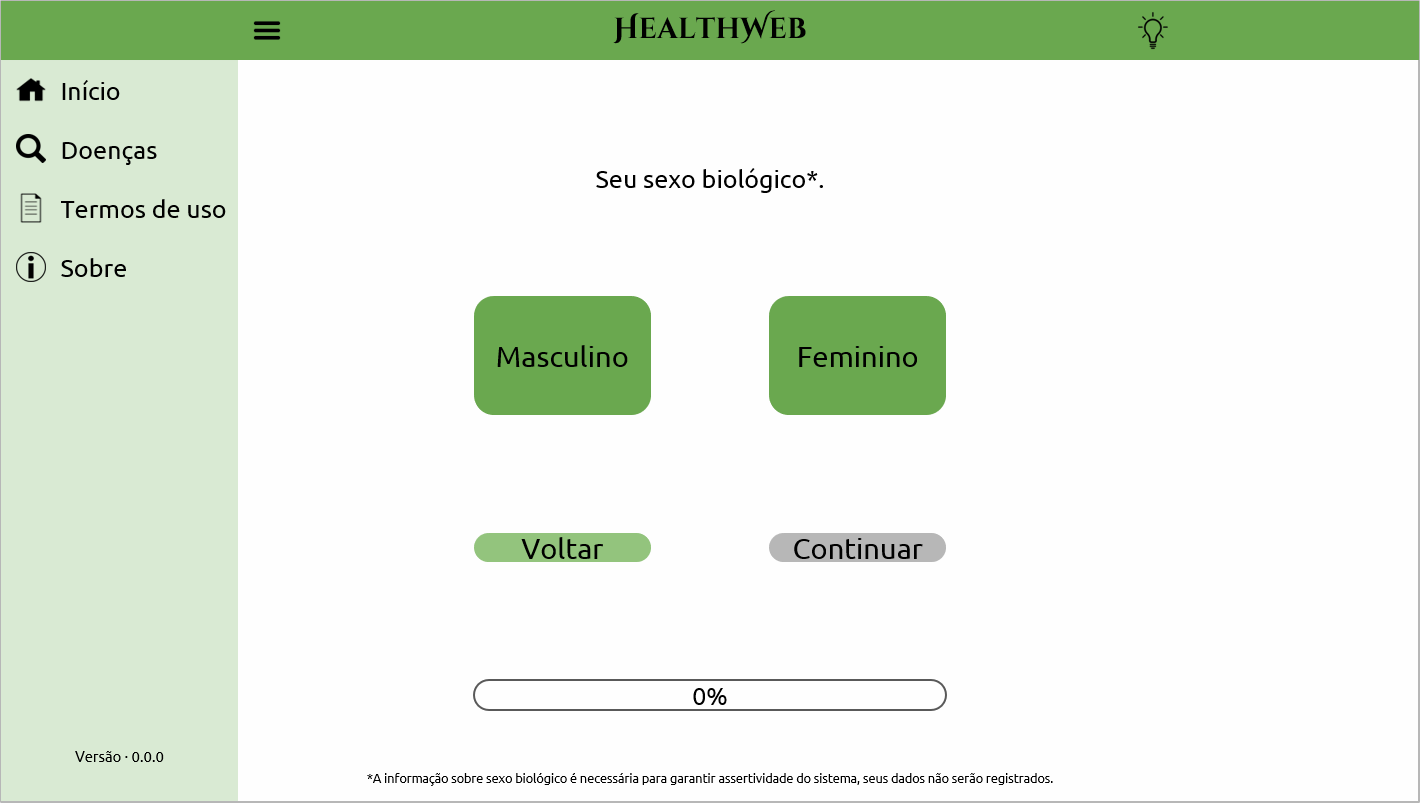
\includegraphics[width=\linewidth]{figure/prototype/desktop/bio_sex.png}
		\caption{Sexo biológico.}
		\label{fig:desktop:bio_sex}
	\end{subfigure}
	\hfill
	\begin{subfigure}{0.49\linewidth}
		\centering
		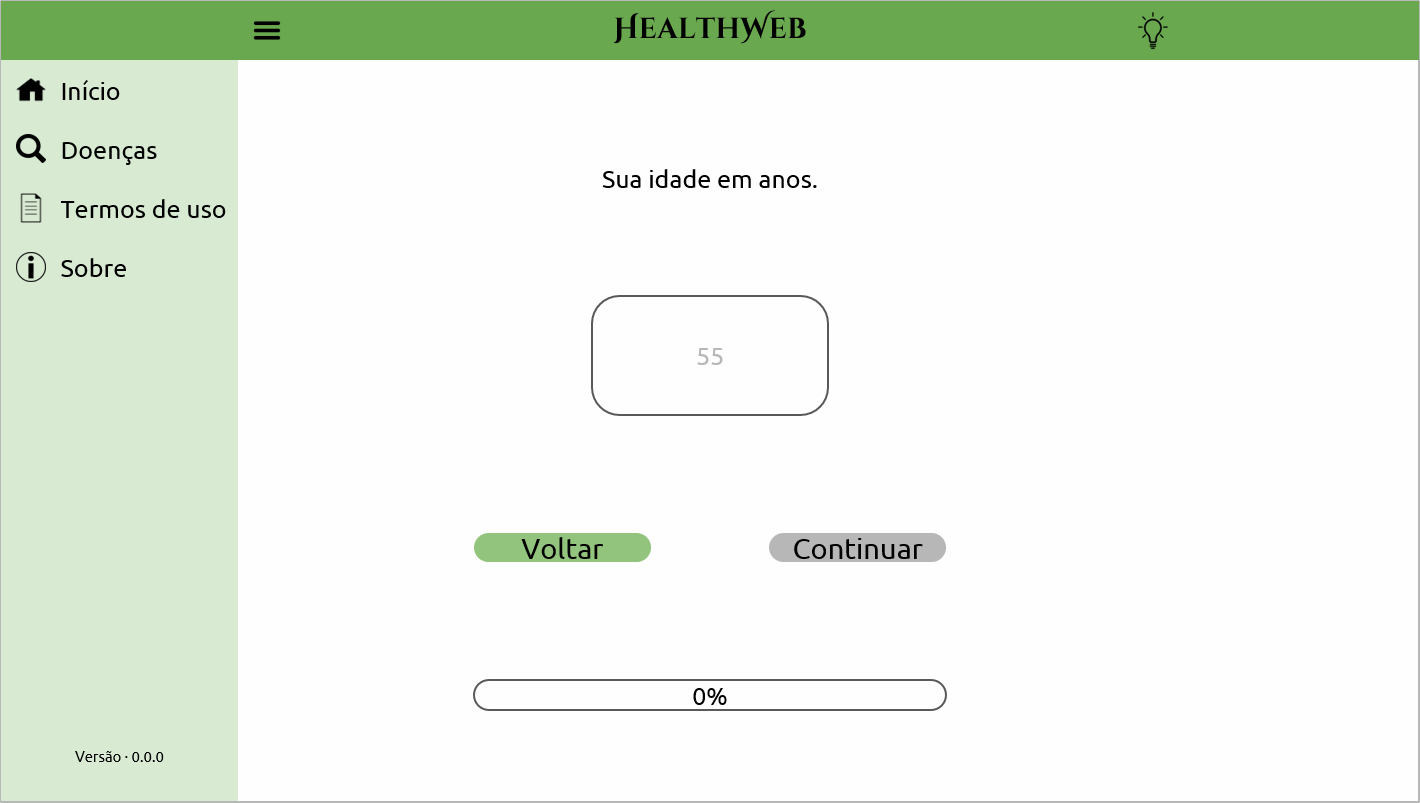
\includegraphics[width=\linewidth]{figure/prototype/desktop/age.png}
		\caption{Idade.}
		\label{fig:desktop:age}
	\end{subfigure}
	\hfill
	\begin{subfigure}{0.49\linewidth}
		\centering
		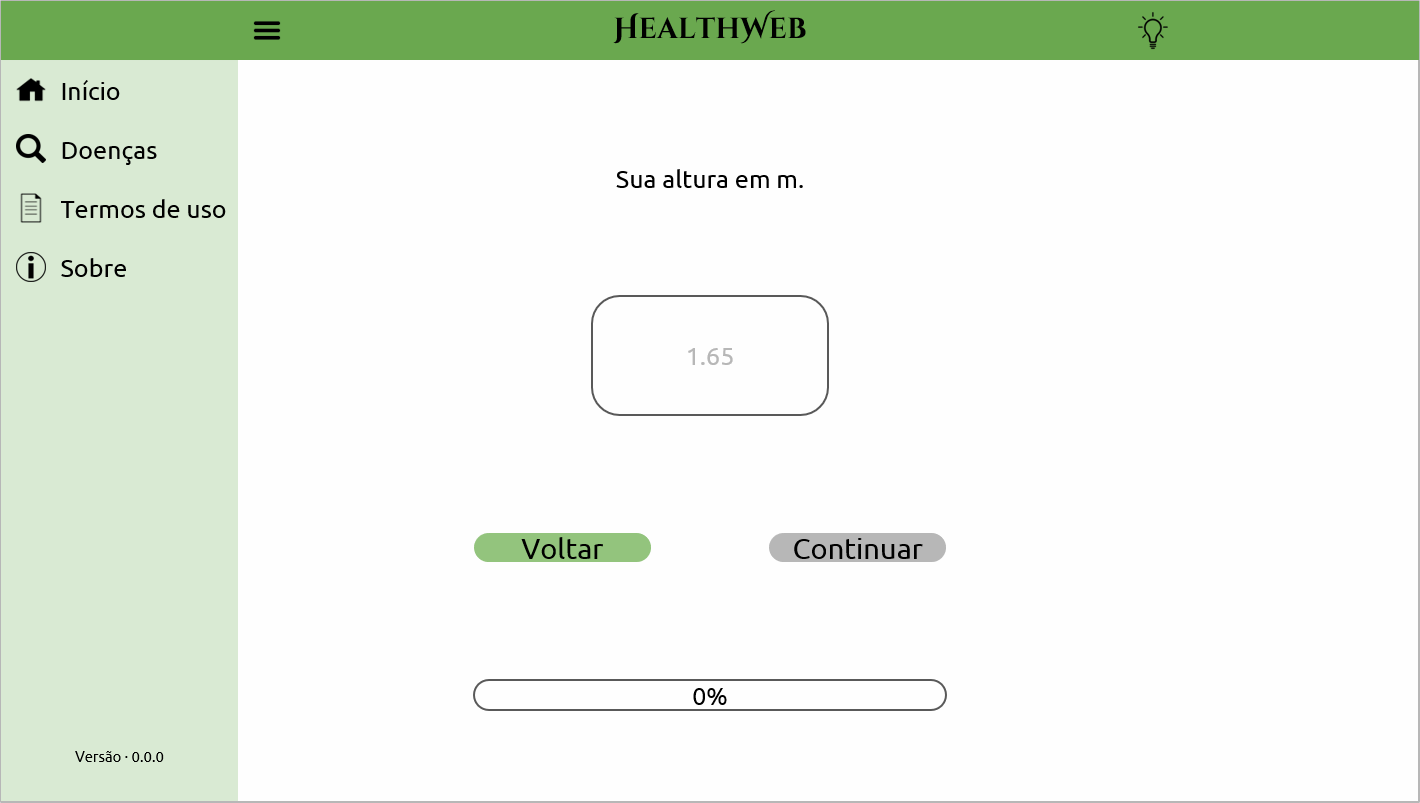
\includegraphics[width=\linewidth]{figure/prototype/desktop/height.png}
		\caption{Altura.}
		\label{fig:desktop:height}
	\end{subfigure}
	\hfill
	\begin{subfigure}{0.49\linewidth}
		\centering
		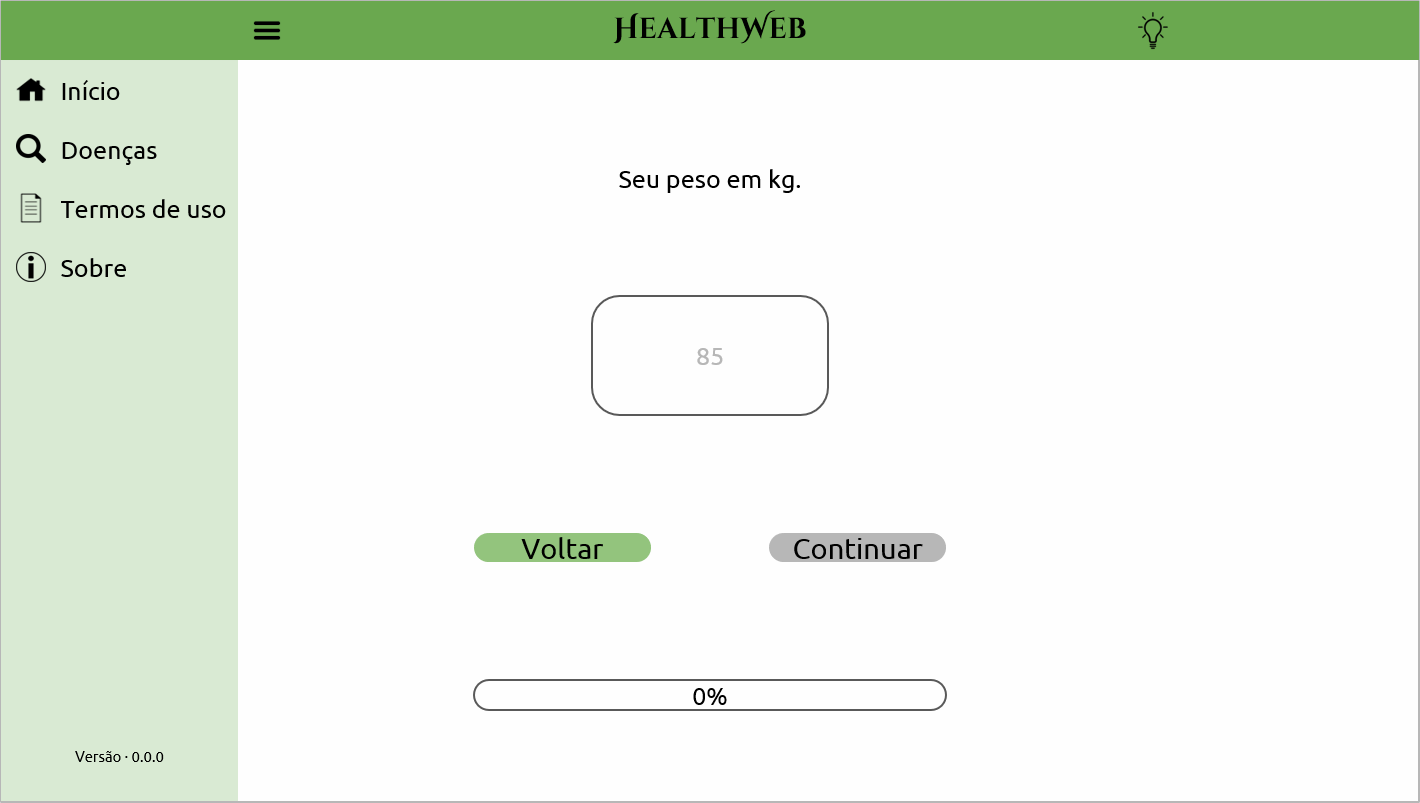
\includegraphics[width=\linewidth]{figure/prototype/desktop/weight.png}
		\caption{Peso.}
		\label{fig:desktop:weight}
	\end{subfigure}
	\caption{Perguntas sobre informações básicas do usuário.}
	\label{fig:desktop:bio_sex_age_height_weight}
\end{figure}

\begin{figure}[htbp]
	\centering
	\begin{subfigure}{0.49\linewidth}
		\centering
		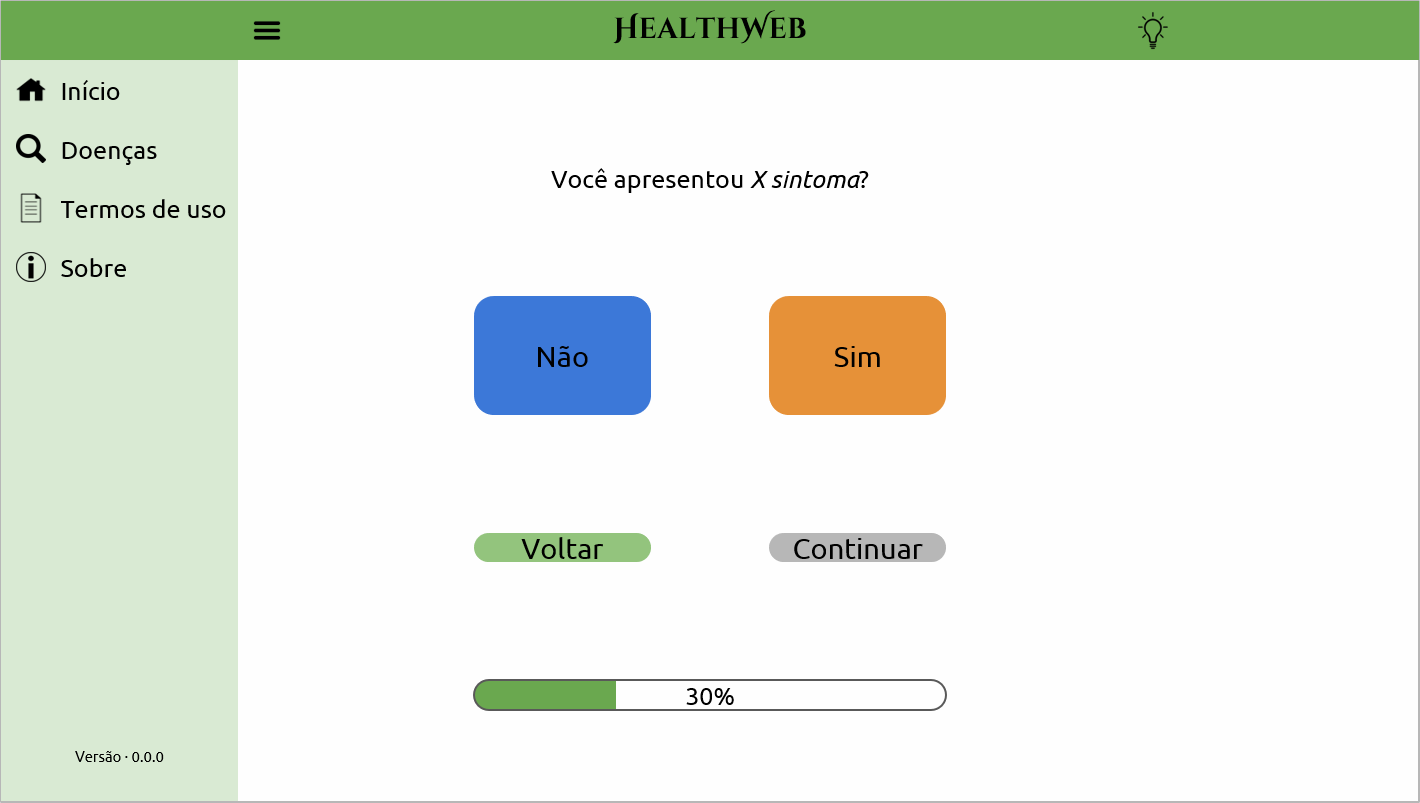
\includegraphics[width=\linewidth]{figure/prototype/desktop/symptom.png}
		\caption{Antes da resposta.}
		\label{fig:desktop:symptom}
	\end{subfigure}
	\linebreak
	\begin{subfigure}{0.49\linewidth}
		\centering
		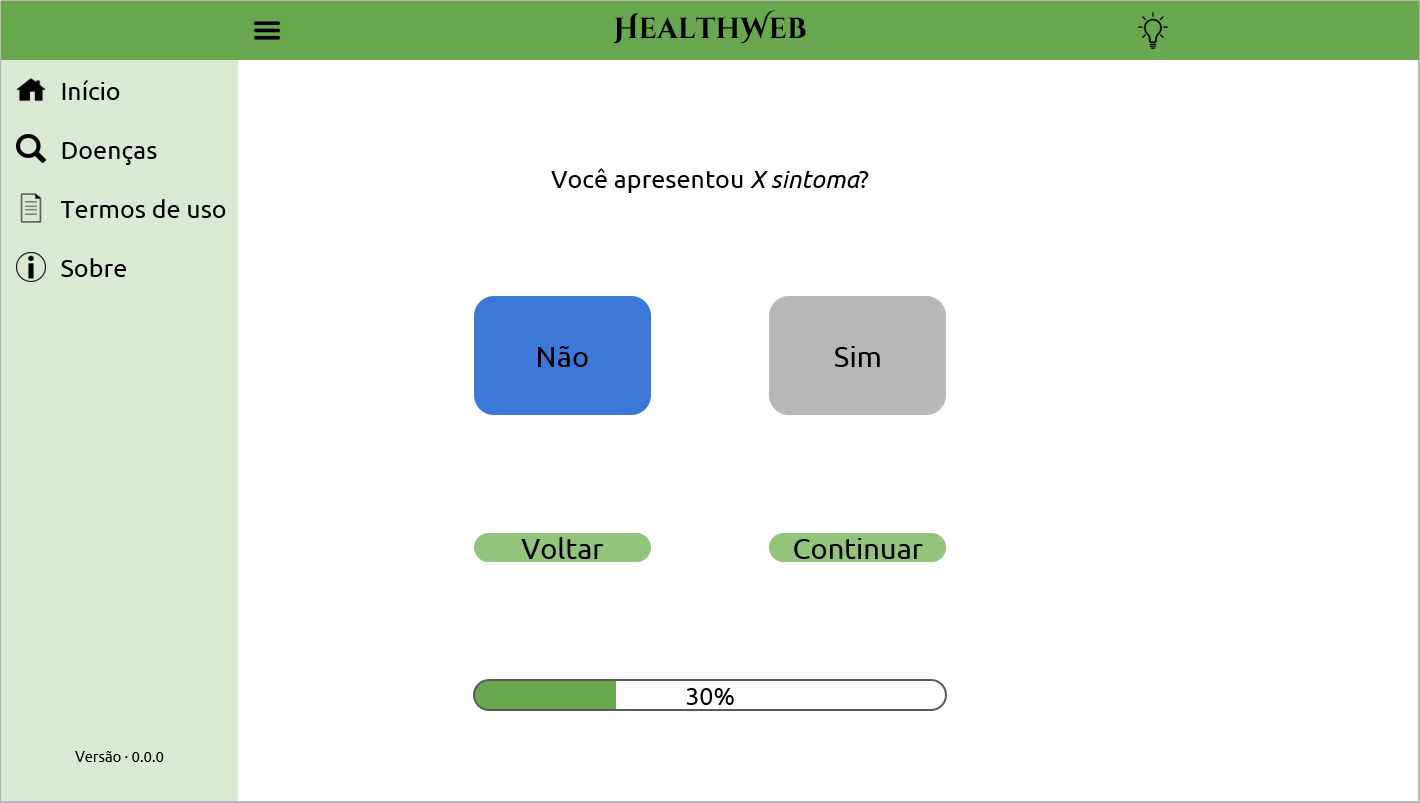
\includegraphics[width=\linewidth]{figure/prototype/desktop/symptom_no.png}
		\caption{Resposta negativa.}
		\label{fig:desktop:symptom_no}
	\end{subfigure}
	\hfill
	\begin{subfigure}{0.49\linewidth}
		\centering
		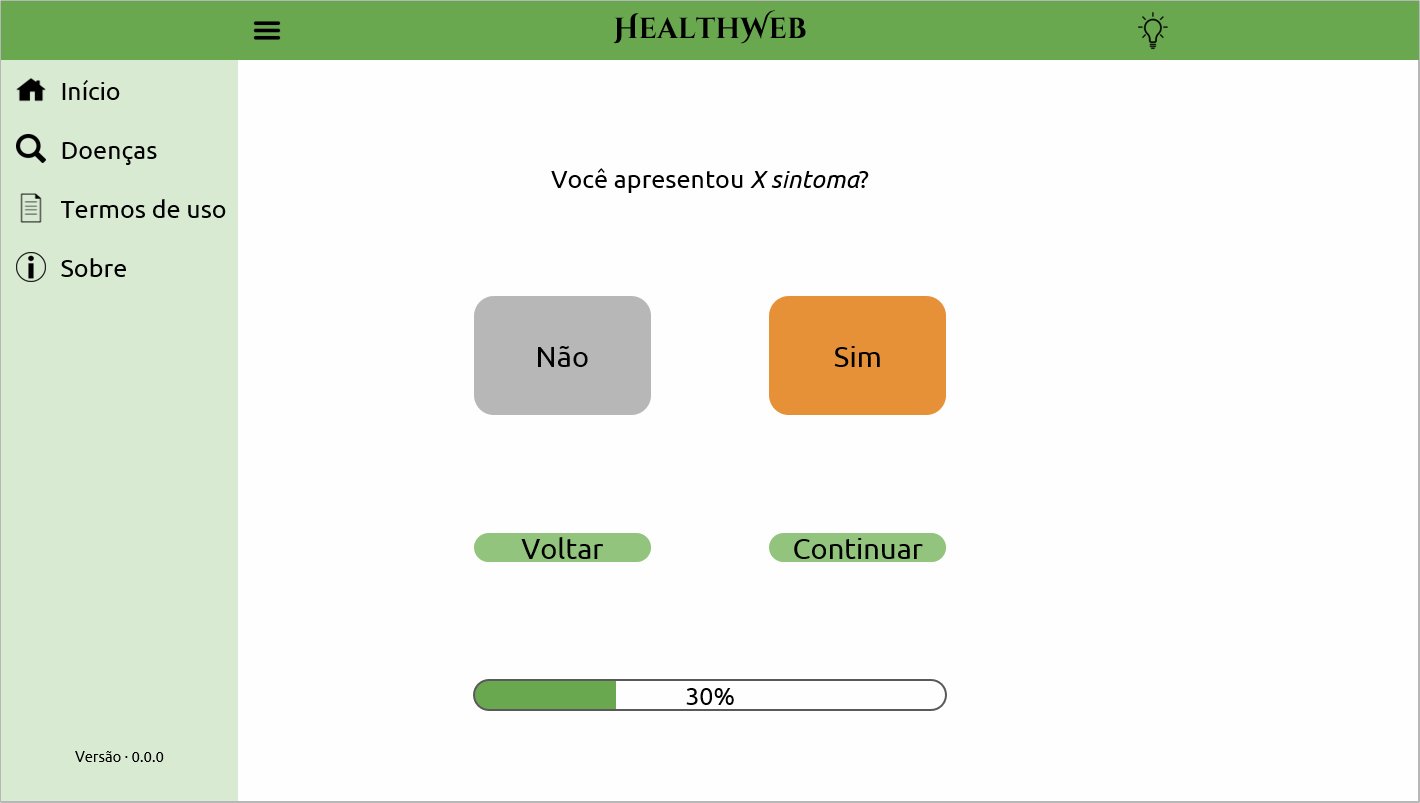
\includegraphics[width=\linewidth]{figure/prototype/desktop/symptom_yes.png}
		\caption{Resposta positiva.}
		\label{fig:desktop:symptom_yes}
	\end{subfigure}
	\hfill
	\caption{Interface durante questionário de sintomas.}
	\label{fig:desktop:symptom_yes_no}
\end{figure}

\begin{figure}[htbp]
	\centering
	\begin{subfigure}{0.49\linewidth}
		\centering
		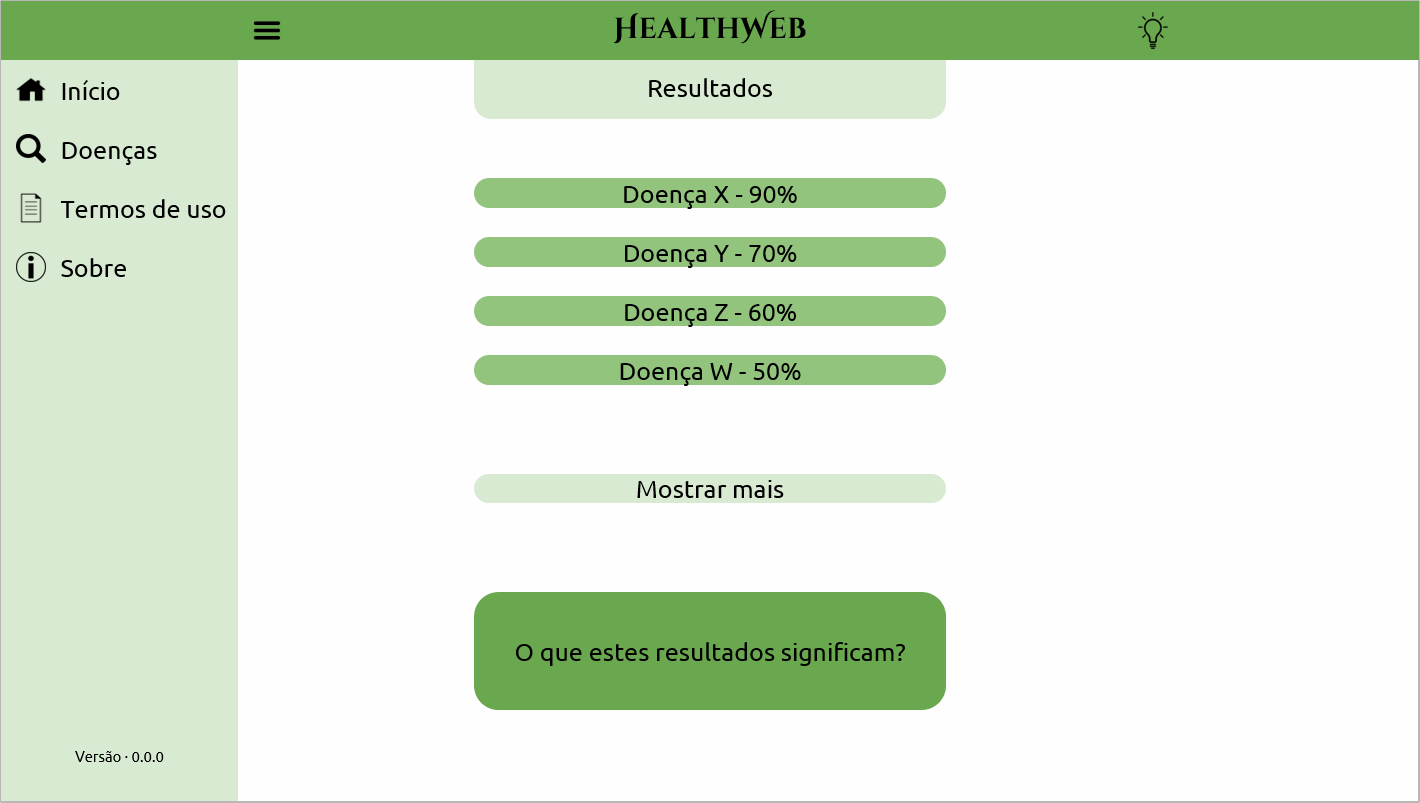
\includegraphics[width=\linewidth]{figure/prototype/desktop/results.png}
		\caption{Resultados.}
		\label{fig:desktop:results}
	\end{subfigure}
	\hfill
	\begin{subfigure}{0.49\linewidth}
		\centering
		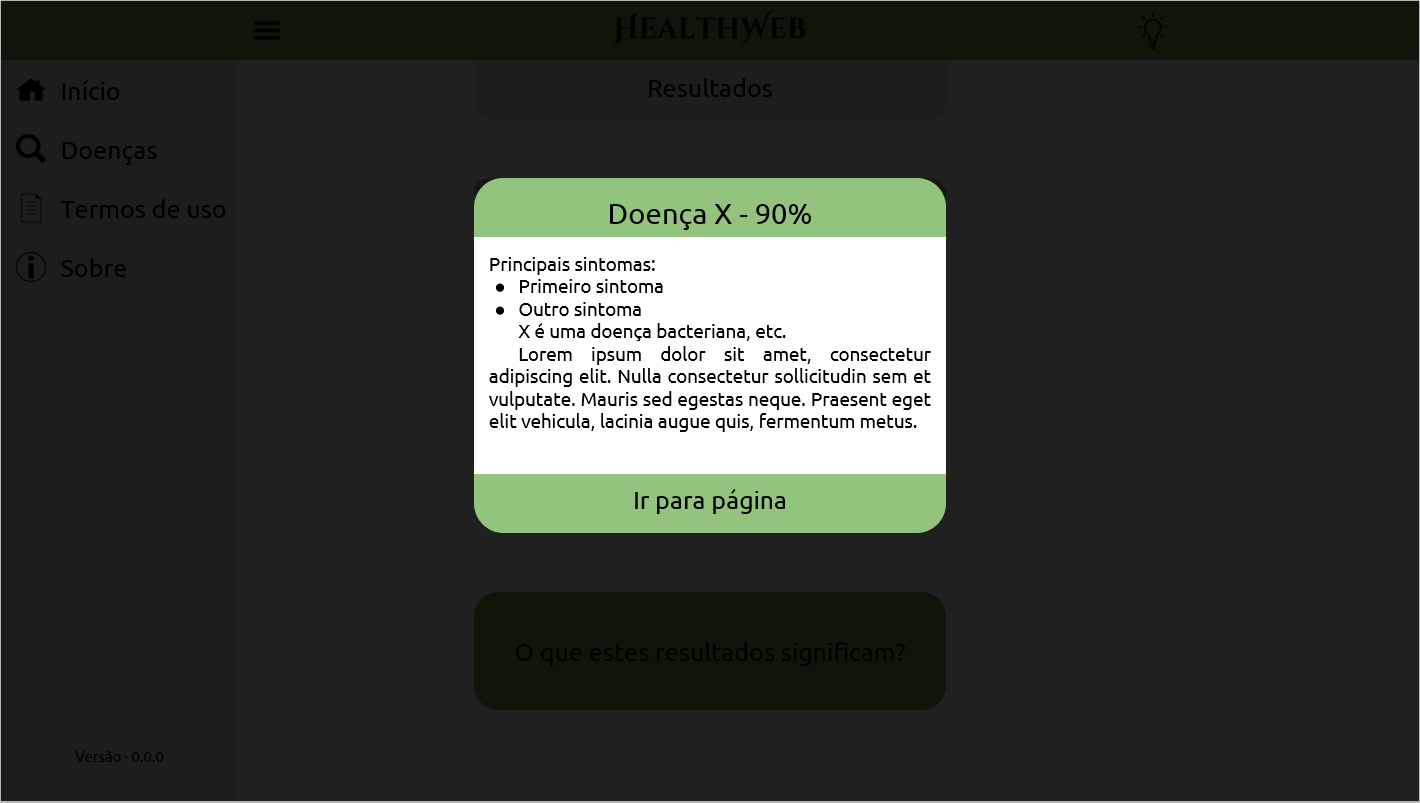
\includegraphics[width=\linewidth]{figure/prototype/desktop/this_disease.png}
		\caption{Resumo sobre doença.}
		\label{fig:desktop:this_disease}
	\end{subfigure}
	\hfill
	\begin{subfigure}{0.49\linewidth}
		\centering
		
\includegraphics[width=\linewidth]{figure/prototype/desktop/disease_page.png}
		\caption{Página sobre doença.}
		\label{fig:desktop:disease_page}
	\end{subfigure}
	\hfill
	\begin{subfigure}{0.49\linewidth}
		\centering
		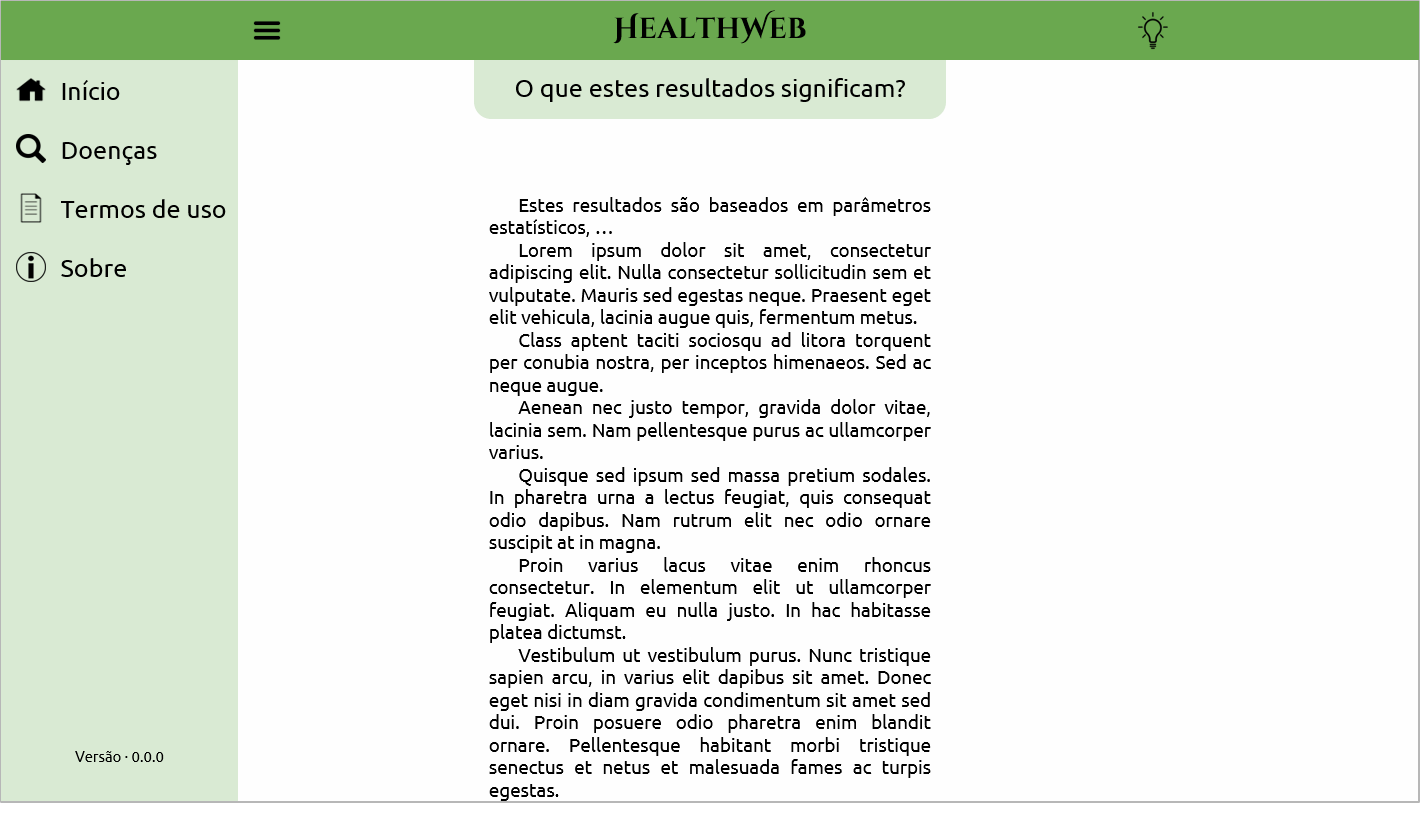
\includegraphics[width=\linewidth]{figure/prototype/desktop/meaning.png}
		\caption{Explicação.}
		\label{fig:desktop:meaning}
	\end{subfigure}
	\caption{Interface de detalhamento e resultados.}
	\label{fig:desktop:results_this_disease_disease_page_meaning}
\end{figure}

\begin{figure}[htbp]
	\centering
	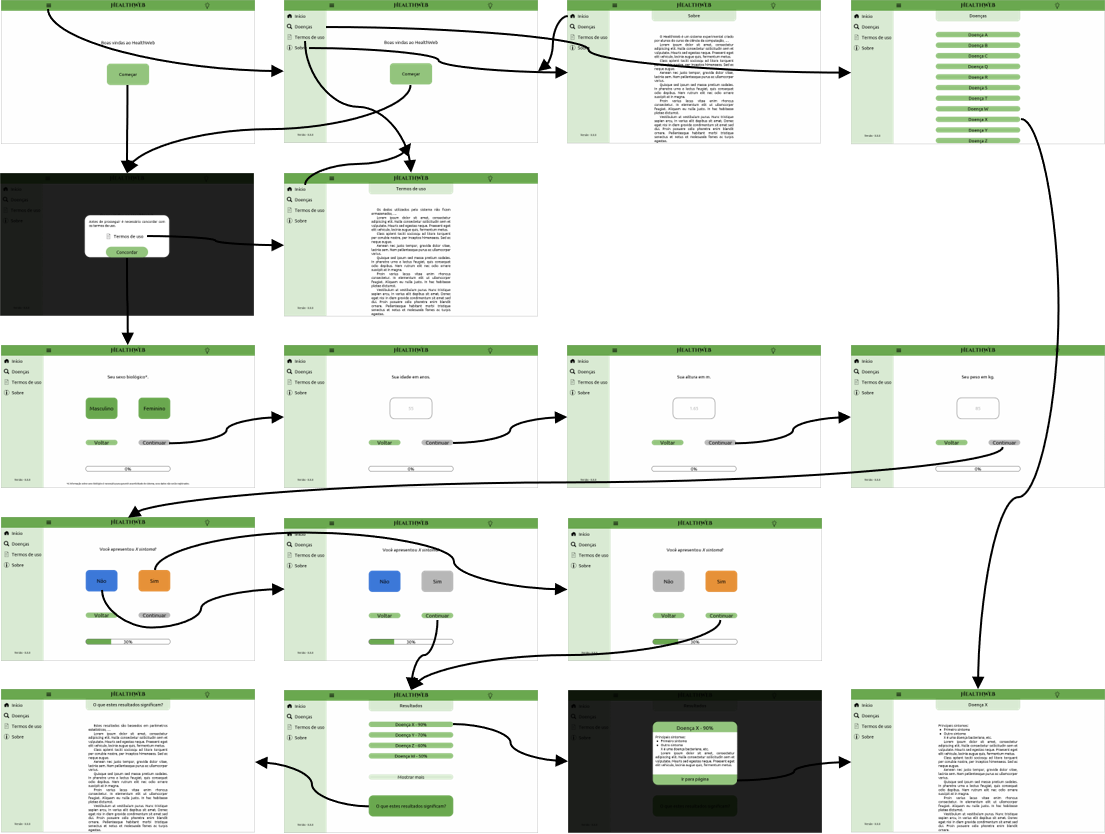
\includegraphics[width=\linewidth]{figure/prototype/desktop/storyboard.png}
	\caption{Storyboard para versão desktop.}
	\label{fig:desktop:story}
\end{figure}